%%*****************************************************************************
%% $Id: started.tex,v 0.00 2008/05/01 17:52:50 gene Exp $
%%*****************************************************************************
%% Author: Gerd Neugebauer
%%-----------------------------------------------------------------------------

\chapter{Getting Started}
%@author Gerd Neugebauer

In this chapter we describe the steps you can take to get \ExBib\ up
and running. We try to use as few as possible premises. Thus it should
be not too hard to get started.

\section{Prerequisites}
%@author Gerd Neugebauer

\subsection{Java}
%@author Gerd Neugebauer

You need to have Java 5\index{Java} or later installed on your
system. You can get Java for a several systems directly from
\url{java.sun.com}. Download and install it according to the
installation instructions for your environment.

To check that you have an appropriate Java on your path you can use
the command \texttt{java} with the argument \texttt{-version}. This
can be seen in the following example:

\lstset{morecomment=[l]{\#}}%
\begin{lstlisting}{morecomment=[l][keywordstyle]{>}}
# java -version
java version "1.5.0_04"
Java(TM) 2 Runtime Environment, Standard Edition (build 1.5.0_04-b05)
Java HotSpot(TM) Client VM (build 1.5.0_04-b05, mixed mode)
#
\end{lstlisting}


\subsection{TEXMF}
%@author Gerd Neugebauer

If you want to use more than the pure \ExBib\ engine, styles can be
inherited from a texmf tree\index{texmf}. \ExBib\ itself does not
contain a full texmf tree. It comes just with some rudimentary files
necessary for testing and getting started. Thus you should have
installed a texmf tree, e.g. from a \TeX Live\index{TeXlive@\TeX Live}
installation. This can be found on the
\href{http://www.ctan.org}{Comprehensive \TeX\ Archive Network
  (CTAN)}\index{CTAN}.

There is no need to install the texmf tree in a special place. You
have to tell \ExBib\ anyhow where it can be found. It is even possible
to work with several texmf trees.

One requirement for the texmf trees is that they have a file database
(\File{ls-R}). \ExBib\ can be configured to work without it, but then
\ExBib\ is deadly slow. Thus you do not really want to try this
alternative.


\section{Getting \ExBib}
%@author Gerd Neugebauer

\subsection{Getting the Installer}
%@author Gerd Neugebauer

The simplest way to get \ExBib\ up and running is to use the \ExBib\ 
installer. This installer\index{installer} is distributed as one file
\File{ExBib-setup.jar}. You can download it from

\begin{quotation}
  \url{http://www.extex.org/download/}
\end{quotation}

If you have got the installer there is no need for you to get the
sources as well. Nevertheless the soruces can be retrieved via
Subversion from
\verb|https://svn.berlios.de/svnroot/repos/extex/trunk/ExBib|.


\section{Installing \ExBib}\label{sec:install}
%@author Gerd Neugebauer

The installation of \ExBib\ works with the \ExBib\ installer. This
installer is named \File{ExBib-setup.jar}. You can start the installer
with the following command line:\index{installer}

\begin{lstlisting}{}
# java -jar ExTeX-setup.jar
\end{lstlisting}

On Windows\index{Windows} with a properly installed Java\index{Java}
you can also start the installer by double-clicking
\texttt{ExBib-setup.jar} in the Explorer\index{Explorer}. This might
work on other windowing systems as well.

\begin{figure}[!h]
  \centering
  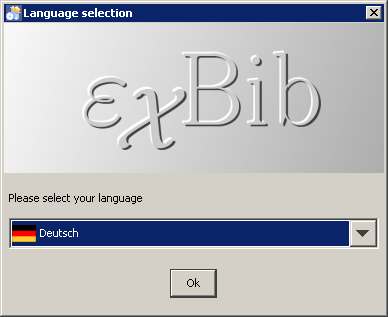
\includegraphics[width=.45\textwidth]{img/inst1}\hfill
  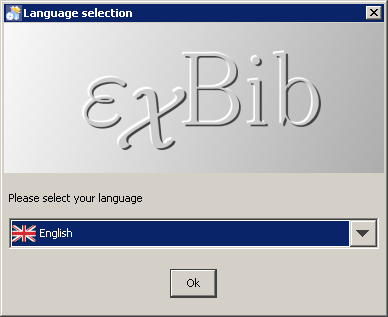
\includegraphics[width=.45\textwidth]{img/inst2}
  \caption{The Language Selection in the Installer}
  \label{fig:inst1}
\end{figure}
The installer provides a graphical user interface with a wizard
guiding you through the installation process. The first dialog is
shown in figure~\ref{fig:inst1}. As you can see you can select one of
several languages for the installation process. This selection just
effects the language used to communicate during the instanllation
process.  Currently the languages English and German are supported.
There might be some more at the time you are performing the
installation.\index{installer!language}\index{language!installer}

Note that the language selection covers the installer only. \ExBib\ 
can be run under different language environments as well. This is
controlled by a setting at run-time. Currently only an English and
a German language binding for \ExBib\ are provided.\index{language}

\begin{figure}[!h]
  \centering
  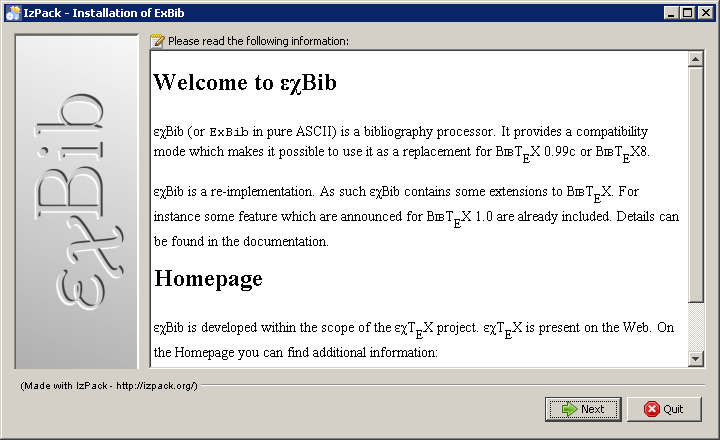
\includegraphics[width=.45\textwidth]{img/inst3}
  \caption{Welcome to \ExBib}
  \label{fig:inst2}
\end{figure}

The next panel shows a welcome message showing what this installer is
about (see figure~\ref{fig:inst2}). Since you are reading this
document there is nothing new for you.

\begin{figure}[!h]
  \centering
  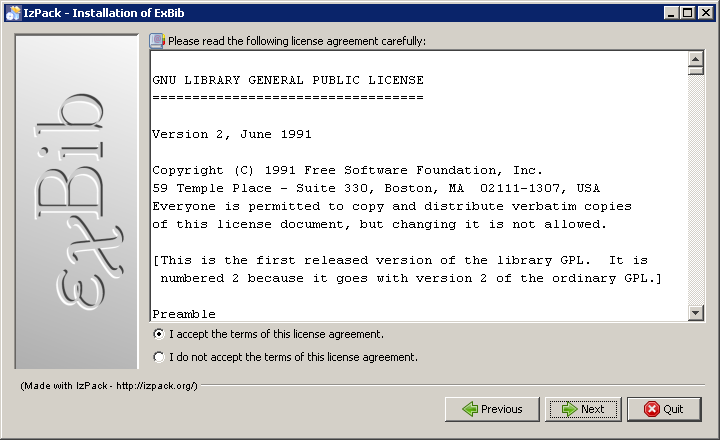
\includegraphics[width=.45\textwidth]{img/inst4}
  \caption{Accepting the Licence}
  \label{fig:inst3}
\end{figure}

Now the license of \ExBib\ is presented (see figure~\ref{fig:inst3}).
It is there to remind you that there is something like a license. You
can not do everything with the software. But the limitations are very
minimalistic. Usually it should not really affect you -- especially
when you are migrating from \BibTeX.

Note that the license is the LGPL. In contrast to the GPL it does not
infect other software build from \ExBib\ or containing it.

\begin{figure}[!h]
  \centering
  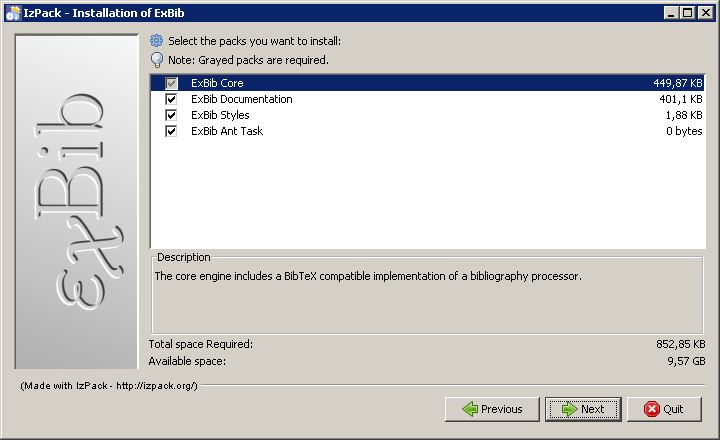
\includegraphics[width=.45\textwidth]{img/inst5}
  \caption{Selecting the Packages}
  \label{fig:inst4}
\end{figure}

Next the packages to be installed can be selected (see
figure~\ref{fig:inst4}). The core packages is needed in any case. Thus
it can not be deselected. The other packages can be freely choosen
from.

Whenever you select a package in the list a short discription of the
package is displayed.

\begin{figure}[!h]
  \centering
  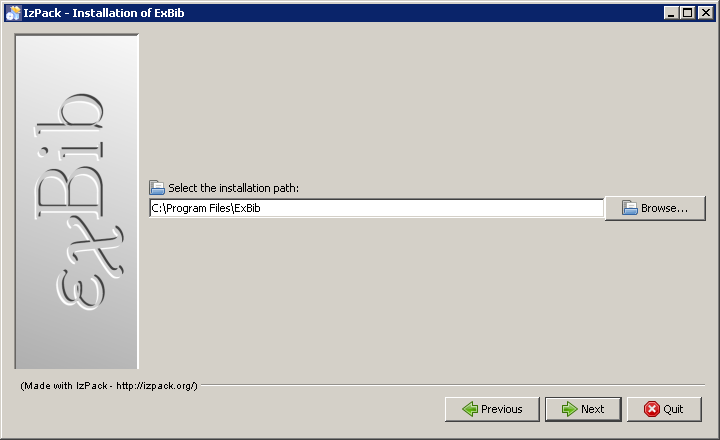
\includegraphics[width=.45\textwidth]{img/inst6}
  \caption{Selecting the Installation Directory}
  \label{fig:inst5}
\end{figure}

Finally the installation directory has to be selected (see
figure~\ref{fig:inst5}). The installation directory (see also
section~\ref{sec:inst.dir}) is the only directory the \ExBib\ 
installer creates files in. Usually is should be separate from other
directories. For instance the value \verb|C:\Program Files\ExBib| on
Windows or \verb|/opt/ExBib| on Unix are sensible values. Nevertheless
the installation can also be performed in your home directory if you
do not have writing permissions in the global directories.

This is the last decision you have to make.

\begin{figure}[!h]
  \centering
  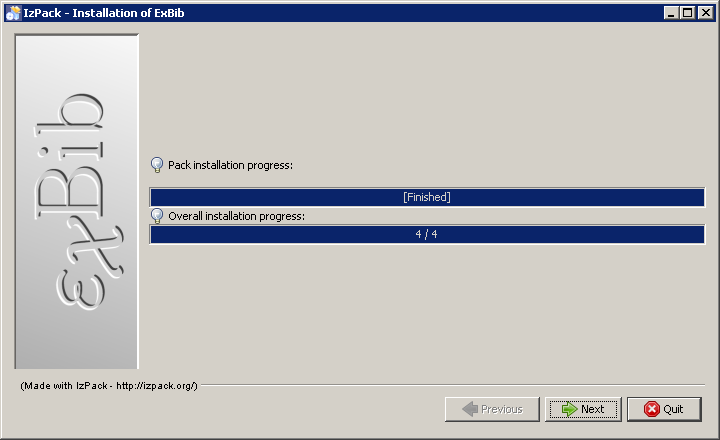
\includegraphics[width=.45\textwidth]{img/inst7}
  \caption{Progress of the Installation}
  \label{fig:inst6}
\end{figure}

Now the installation is performed. A progress panel is shown during
the installation (see figure~\ref{fig:inst6}). As a result the
installation directory is created and filled (see also
section~\ref{sec:inst.dir})

\begin{figure}[!h]
  \centering
  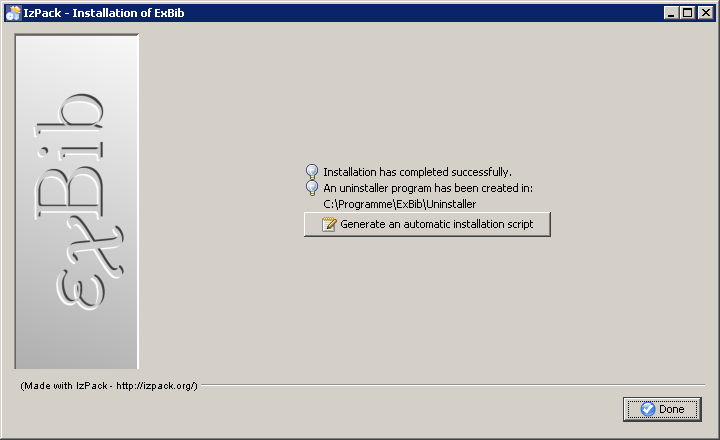
\includegraphics[width=.45\textwidth]{img/inst8}
  \caption{Saving the Installation Settings}
  \label{fig:inst7}
\end{figure}

When the installation is completed you get the chance to save the
settings for unattended replay (see figure~\ref{fig:inst7}). See
section~\ref{sec:replay} for details.


Finally you have to make sure that the executables \Prog{exbib} or
\Prog{exbib.bat} are on your path for executables.\index{path} This
can be achieved by modifying the environment variable \verb|PATH| in a
Unix environment or setting \verb|path| in the system settings on
Windows.


\subsection{The Installation Directory}\label{sec:inst.dir}
%@author Gerd Neugebauer

During the installation you choose a directory where \ExBib\ lives.
This is called the installation directory. An example of the contents of the
installation directory can be seen in figure~\ref{fig:inst.dir}.

\begin{figure}[!h]
  \centering
\begin{DirList}{200pt}{250pt}
  \TOPDIR(0,30){ExBib}
  \DIR(3,28)2{Uninstaller}
  \FILE(6,26)2{uninstaller.jar}
  \DIR(3,24){4.75}{bin}
  \FILE(6,22)2{exbib}
  \FILE(6,20){2.5}{exbib.bat}
  \FILE(6,18){2.5}{exbibutil}
  \FILE(6,16){2.5}{exbibutil.bat}
  \DIR(3,14){10.75}{doc}
  \FILE(6,12)2{exbib-manual.pdf}
  \DIR(3,10){4.75}{lib}
  \FILE(6,8){2}{ExBib-core.jar}
  \FILE(6,6){2.5}{ExBib-Main.jar}
  \FILE(6,4){2.5}{ExBib-styles.jar}
  \FILE(6,2){2.5}{ExTeX-resource.jar}
  \FILE(3,0){10.75}{LICENSE.txt}
\end{DirList}
  \caption{The Installation Directory}

  \label{fig:inst.dir}
\end{figure}

The directory \File{Uninstaller} contains the uninstaller. It can be
used to get rid of \ExBib\ -- even when I don't know why you should
want to. For details see section~\ref{sec:uninst}

The directory \File{bin} contains the binaries. This directory should
be put onto the path for executables. Note that currently all
executables are installed on any platform. On Windows the programs
without extension can be useful within the cygwin world. On Unix the
files with the extension \verb|.bat| can be simply ignored.

The directory \File{doc} contains documentation if the documentation
package has been selected during the installation.

The directory \File{lib} contains the libraries used by \ExBib.


\subsection{Replaying an Installation}\label{sec:replay}
%@author Gerd Neugebauer

Sometimes it is desirable to perform an installation on several
similar machines. This means that the answers to the questions in the
installer are the same. This process can be automated.

In figure~\ref{fig:inst7} you can see the last screen of the
installer. Here you have the possibility to select the button
``Generate an automatic installation script''. This produces an XML
file which can be passed to the installer to avoid the
dialogs.\index{installer}\index{installation script}

Suppose you have named the file \texttt{replay.xml} in the file
selector which pops up when the button has been pressed. Then you can
replay the installation with the following command invocation:

\begin{lstlisting}{}
# java -jar ExBib-setup.jar replay.xml
\end{lstlisting}

This supposes that the two files \File{ExTeX-setup.jar} and
\texttt{replay.xml} are in the current directory.

\subsection{Uninstalling \ExBib}\label{sec:uninst}
%@author Gerd Neugebauer

The files installed by the installer (see section~\ref{sec:install})
can be removed from the system. For this purpose an uninstaller is
provided in the subdirectory \File{Uninstaller} of the \ExBib\
installation directory. It is named \File{uninstaller.jar}. It can be
invoked by double clicking or invoking it on the command line as follows:

\begin{lstlisting}{}
# java -jar uninstaller.jar
\end{lstlisting}

\begin{figure}[!h]
  \centering
  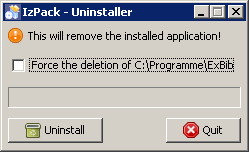
\includegraphics[width=.45\textwidth]{img/uninst1}
  \caption{Confirming the Uninstallation}
  \label{fig:uninst1}
\end{figure}

When the uninstaller starts it asks for configmation (see
figure~\ref{fig:uninst1}). Nothing is changed before the confirmation
is given.

\begin{figure}[!h]
  \centering
  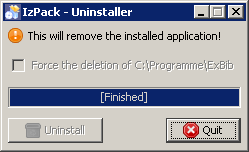
\includegraphics[width=.45\textwidth]{img/uninst2}
  \caption{The Uninstaller Finished}
  \label{fig:uninst1}
\end{figure}

The uninstaller shows a progress bar (see figure~\ref{fig:uninst2}).
When the uninstaller has finished its work all files and directories
installed with the installer have been removed. Modified and other
files are left untouched.

You can uninstall \ExBib\ by simply removing the installation
directory. But this is unsave since all local modification are lost as
well.


%------------------------------------------------------------------------------
\section{Running \ExBib}
%@author Gerd Neugebauer

Currently \ExBib\ can be run from the command line. In this respect it
is more or less identical to \BibTeX\ and can be used as a plug-in
replacement.

\iffalse%-----------------------------------------

The following sample show a simple invocation of \ExBib\ without any
command line arguments.

{\lstset{morecomment=[l]{*}}%
\begin{lstlisting}{}
# exbib
This is exbib, Version 0.0 (TeX compatibility mode)
**\relax

*\end

No pages of output.
Transcript written on ./texput.log.
\end{lstlisting}}

In this case \ExTeX\ enters interaction with the user and asks for an
input file. This is indicated by the two asterisks. We have entered
\macro{relax} here to indicate that we are not willing to pass in a
file name. The \ExTeX\ system asks us to enter some command --
indicted by the single asterisk. Here we have entered \macro{end} to
indicate that we want to finish the processing. Thus \ExTeX\ 
terminates normally.

\INCOMPLETE

{\lstset{morecomment=[l]{*}}%
\begin{lstlisting}{}
# extex plain
This is ExTeX, Version 0.0 (TeX compatibility mode)
(plain Preloading the plain format: codes, registers, parameters, fonts,
more fonts, macros, math definitions, output routines, hyphenation(hyphen))
*\dump
Beginning to dump on file plain.fmt

*\end

No pages of output.
Transcript written on ./plain.log.
\end{lstlisting}}


\subsection{Command Line Parameters}
%@author Gerd Neugebauer

The invocation of the executable \Prog{extex} can be controlled by
large number of command line arguments. Those command line arguments
are described in the following list:

\begin{description}
\item[\Arg{code}]\ \\
  This parameter contains \ExTeX\ code to be executed directly. The
  execution is performed after any code specified in an input file. On
  the command line the code has to start with a backslash. This
  restriction does not hold for the property settings.

  This command line argument sets the property \Property{extex.code}
  
\item[\Arg{file}]\ \\
  This parameter contains the file to read from. A file name may not
  start with a backslash or an ambercent. It has no default.

  This command line argument sets the property \Property{extex.file}.
  
\item[\CLI{-} \Arg{file}]\ \\
  This parameter terminates the normal processing of arguments. The
  next argument -- if present -- is interpreted as input file. With
  this construction it is possible to process an input file which
  starts with one of the special characters \verb|\| or \verb|&|.

  This command line argument sets the property \Property{extex.file}
  if a file argument is present.

\item[\CLI{configuration} \Arg{resource}]\ \\
  This parameter contains the name of the configuration resource to
  use. This configuration resource is sought on the class path.
  
  This command line argument sets the property \Property{extex.config}.
  
\item[\CLI{copyright}]\ \\
  This command line option produces a copyright notice on the standard
  output stream and terminates the program afterwards.

\item[\tt\&\Arg{format}]\index{\&}
\item[\CLI{fmt} \Arg{format}]\ \\
  This parameter contains the name of the format to read. An empty
  string denotes that no format should be read. This is the default.

  This command line argument sets the property \Property{extex.format}.
  
\item[\CLI{debug} \Arg{spec}]\ \\
  This command line parameter can be used to instruct the program to
  produce debugging output of several kinds. The debug output is
  written to the log file. The specification \Arg{spec} is interpreted
  left to right. Each character is interpreted according to the
  following table:

  \begin{tabular}{lp{.4\textwidth}l}\toprule
    \textit{Spec}& \textit{Description}& \textit{See} \\\midrule
    F& 	This specifier contains the indicator whether or not to trace
    the searching for input files. & 	\Property{extex.trace.input.files}\\
    f& 	This specifier contains the indicator whether or not to trace
    the searching for font files.&      \Property{extex.trace.font.files}\\
    M& 	This specifier contains the indicator whether or not to trace
    the execution of macros.&	 	\Property{extex.trace.macros}\\
    T& 	This specifier contains the indicator whether or not to trace
    the work of the tokenizer.& 	\Property{extex.trace.tokenizer}\\
    \bottomrule
  \end{tabular}

  The following example shows a possible invocation with this
  parameter: 
\begin{lstlisting}{}
# extex -debug FfMT abc.tex
This is ExTeX, Version 0.0 (TeX compatibility mode)
...
\end{lstlisting}
  
\item[\CLI{halt-on-error}]\ \\
  This parameter contains the indicator whether the processing should
  halt after the first error which has been encountered.

  This command line argument sets the property \Property{extex.halt.on.error}.
  
\item[\CLI{help}]\ \\
  This command line option produces a short usage description on the
  standard output stream and terminates the program afterwards.
  
\item[\CLI{ini}]\ \\
  If set to true then act as ini\TeX.\index{initex@ini\TeX} In this
  case no format has to be preloaded. All parameters are set to the
  "`factory settings"'.

  This command line argument sets the property \Property{extex.ini}.

  The following example shows a possible invocation with this
  parameter: 
\begin{lstlisting}{}
# extex -ini abc.tex
This is ExTeX, Version 0.0 (TeX compatibility mode)
...
\end{lstlisting}
  
\item[\CLI{interaction} \Arg{mode}]\ \\
  This parameter contains the interaction mode. possible values are
  the numbers 0\dots3 and the symbolic names \Mode{batchmode} (0),
  \Mode{nonstopmode} (1), \Mode{scrollmode} (2), and
  \Mode{errorstopmode} (3).

  This command line argument sets the property \Property{extex.interaction}.
  
  The following example shows a possible invocation with this
  parameter:
\begin{lstlisting}{}
# extex -interaction batchmode abc.tex
This is ExTeX, Version 0.0 (TeX compatibility mode)
...
\end{lstlisting}

\item[\CLI{job-name} \Arg{name}]\ \\
  This parameter contains the name of the job. It is overwritten if a
  file is given to read from. In this case the base name of the input
  file is used instead.

  This command line argument sets the property \Property{extex.jobname}.
  
\item[\CLI{language} \Arg{language}]\ \\
  This parameter contains the name of the locale to be used for the
  messages.

  This command line argument sets the property \Property{extex.lang}.
  
\item[\CLI{output} \Arg{format}]\ \\
  This parameter contains the output format. This logical name is
  resolved via the configuration.

  This command line argument sets the property \Property{extex.output}.

  The following example shows a possible invocation with this
  parameter: 
\begin{lstlisting}{}
# extex -output pdf abc.tex
This is ExTeX, Version 0.0 (TeX compatibility mode)
\end{lstlisting}
  
\item[\CLI{progname} \Arg{name}]\ \\
  This parameter can be used to overrule the name of the program shown
  in the banner and the version information.  The following example
  shows a possible invocation and the resulting output:

\begin{lstlisting}{}
# extex -progname XeTxE -version
This is XeTxE, Version 0.0 (1.4.2_06)
#
\end{lstlisting}

  This command line argument sets the property \Property{extex.progname}.
  
\item[\CLI{texinputs} \Arg{path}]\ \\
  This parameter contains the additional directories for searching
  \ExTeX\ input files.  The directories are separated by the
  system-dependant separator.  This separator is a colon (\verb|:|) on
  Unix\index{Unix} and the semicolon (\verb|;|) on
  Windows\index{Windows}.
  
  This command line argument sets the property
  \Property{extex.texinputs}.
  
\item[\CLI{texmfoutputs} \Arg{dir}]\ \\
  This parameter contains the name of the property for the fallback if
  the output directory fails to be writable.
  
  This command line argument sets the property
  \Property{extex.outputdir.fallback}.
  
\item[\CLI{texoutputs} \Arg{dir}]\ \\
  This parameter contain the directory where output files should be
  created.

  This command line argument sets the property \Property{extex.outputdir}.
  
\item[\CLI{version}]\ \\
  This command line parameter forces that the version information is
  written to standard output and the program is
  terminated.\index{version} The version of \ExTeX\ is shown and the
  version of the Java engine\index{Java} in parentheses. The following
  example shows a possible invocation and the resulting output:

\begin{lstlisting}{}
# extex -version
This is ExTeX, Version 0.0 (1.4.2_06)
#
\end{lstlisting}
\end{description}

Command line parameters can be abbreviated up to a unique prefix --
and sometimes even more. Thus the following invocations are
equivalent:

\begin{verbatim}
  extex -v
  extex -ve
  extex -ver
  extex -vers
  extex -versi
  extex -versio
  extex -version  
\end{verbatim}

\fi%-----------------------------------------

\endinput
%
% Local Variables: 
% mode: latex
% TeX-master: "../exbib-users"
% End: 
